% Options for packages loaded elsewhere
\PassOptionsToPackage{unicode}{hyperref}
\PassOptionsToPackage{hyphens}{url}
%
\documentclass[
]{article}
\usepackage{amsmath,amssymb}
\usepackage{iftex}
\ifPDFTeX
  \usepackage[T1]{fontenc}
  \usepackage[utf8]{inputenc}
  \usepackage{textcomp} % provide euro and other symbols
\else % if luatex or xetex
  \usepackage{unicode-math} % this also loads fontspec
  \defaultfontfeatures{Scale=MatchLowercase}
  \defaultfontfeatures[\rmfamily]{Ligatures=TeX,Scale=1}
\fi
\usepackage{lmodern}
\ifPDFTeX\else
  % xetex/luatex font selection
\fi
% Use upquote if available, for straight quotes in verbatim environments
\IfFileExists{upquote.sty}{\usepackage{upquote}}{}
\IfFileExists{microtype.sty}{% use microtype if available
  \usepackage[]{microtype}
  \UseMicrotypeSet[protrusion]{basicmath} % disable protrusion for tt fonts
}{}
\makeatletter
\@ifundefined{KOMAClassName}{% if non-KOMA class
  \IfFileExists{parskip.sty}{%
    \usepackage{parskip}
  }{% else
    \setlength{\parindent}{0pt}
    \setlength{\parskip}{6pt plus 2pt minus 1pt}}
}{% if KOMA class
  \KOMAoptions{parskip=half}}
\makeatother
\usepackage{xcolor}
\usepackage[margin=1in]{geometry}
\usepackage{color}
\usepackage{fancyvrb}
\newcommand{\VerbBar}{|}
\newcommand{\VERB}{\Verb[commandchars=\\\{\}]}
\DefineVerbatimEnvironment{Highlighting}{Verbatim}{commandchars=\\\{\}}
% Add ',fontsize=\small' for more characters per line
\usepackage{framed}
\definecolor{shadecolor}{RGB}{248,248,248}
\newenvironment{Shaded}{\begin{snugshade}}{\end{snugshade}}
\newcommand{\AlertTok}[1]{\textcolor[rgb]{0.94,0.16,0.16}{#1}}
\newcommand{\AnnotationTok}[1]{\textcolor[rgb]{0.56,0.35,0.01}{\textbf{\textit{#1}}}}
\newcommand{\AttributeTok}[1]{\textcolor[rgb]{0.13,0.29,0.53}{#1}}
\newcommand{\BaseNTok}[1]{\textcolor[rgb]{0.00,0.00,0.81}{#1}}
\newcommand{\BuiltInTok}[1]{#1}
\newcommand{\CharTok}[1]{\textcolor[rgb]{0.31,0.60,0.02}{#1}}
\newcommand{\CommentTok}[1]{\textcolor[rgb]{0.56,0.35,0.01}{\textit{#1}}}
\newcommand{\CommentVarTok}[1]{\textcolor[rgb]{0.56,0.35,0.01}{\textbf{\textit{#1}}}}
\newcommand{\ConstantTok}[1]{\textcolor[rgb]{0.56,0.35,0.01}{#1}}
\newcommand{\ControlFlowTok}[1]{\textcolor[rgb]{0.13,0.29,0.53}{\textbf{#1}}}
\newcommand{\DataTypeTok}[1]{\textcolor[rgb]{0.13,0.29,0.53}{#1}}
\newcommand{\DecValTok}[1]{\textcolor[rgb]{0.00,0.00,0.81}{#1}}
\newcommand{\DocumentationTok}[1]{\textcolor[rgb]{0.56,0.35,0.01}{\textbf{\textit{#1}}}}
\newcommand{\ErrorTok}[1]{\textcolor[rgb]{0.64,0.00,0.00}{\textbf{#1}}}
\newcommand{\ExtensionTok}[1]{#1}
\newcommand{\FloatTok}[1]{\textcolor[rgb]{0.00,0.00,0.81}{#1}}
\newcommand{\FunctionTok}[1]{\textcolor[rgb]{0.13,0.29,0.53}{\textbf{#1}}}
\newcommand{\ImportTok}[1]{#1}
\newcommand{\InformationTok}[1]{\textcolor[rgb]{0.56,0.35,0.01}{\textbf{\textit{#1}}}}
\newcommand{\KeywordTok}[1]{\textcolor[rgb]{0.13,0.29,0.53}{\textbf{#1}}}
\newcommand{\NormalTok}[1]{#1}
\newcommand{\OperatorTok}[1]{\textcolor[rgb]{0.81,0.36,0.00}{\textbf{#1}}}
\newcommand{\OtherTok}[1]{\textcolor[rgb]{0.56,0.35,0.01}{#1}}
\newcommand{\PreprocessorTok}[1]{\textcolor[rgb]{0.56,0.35,0.01}{\textit{#1}}}
\newcommand{\RegionMarkerTok}[1]{#1}
\newcommand{\SpecialCharTok}[1]{\textcolor[rgb]{0.81,0.36,0.00}{\textbf{#1}}}
\newcommand{\SpecialStringTok}[1]{\textcolor[rgb]{0.31,0.60,0.02}{#1}}
\newcommand{\StringTok}[1]{\textcolor[rgb]{0.31,0.60,0.02}{#1}}
\newcommand{\VariableTok}[1]{\textcolor[rgb]{0.00,0.00,0.00}{#1}}
\newcommand{\VerbatimStringTok}[1]{\textcolor[rgb]{0.31,0.60,0.02}{#1}}
\newcommand{\WarningTok}[1]{\textcolor[rgb]{0.56,0.35,0.01}{\textbf{\textit{#1}}}}
\usepackage{graphicx}
\makeatletter
\def\maxwidth{\ifdim\Gin@nat@width>\linewidth\linewidth\else\Gin@nat@width\fi}
\def\maxheight{\ifdim\Gin@nat@height>\textheight\textheight\else\Gin@nat@height\fi}
\makeatother
% Scale images if necessary, so that they will not overflow the page
% margins by default, and it is still possible to overwrite the defaults
% using explicit options in \includegraphics[width, height, ...]{}
\setkeys{Gin}{width=\maxwidth,height=\maxheight,keepaspectratio}
% Set default figure placement to htbp
\makeatletter
\def\fps@figure{htbp}
\makeatother
\setlength{\emergencystretch}{3em} % prevent overfull lines
\providecommand{\tightlist}{%
  \setlength{\itemsep}{0pt}\setlength{\parskip}{0pt}}
\setcounter{secnumdepth}{-\maxdimen} % remove section numbering
\ifLuaTeX
  \usepackage{selnolig}  % disable illegal ligatures
\fi
\IfFileExists{bookmark.sty}{\usepackage{bookmark}}{\usepackage{hyperref}}
\IfFileExists{xurl.sty}{\usepackage{xurl}}{} % add URL line breaks if available
\urlstyle{same}
\hypersetup{
  pdftitle={TP modèles linéaires - Partie 1},
  hidelinks,
  pdfcreator={LaTeX via pandoc}}

\title{TP modèles linéaires - Partie 1}
\author{}
\date{\vspace{-2.5em}4modIA - 2023-2024}

\begin{document}
\maketitle

{
\setcounter{tocdepth}{4}
\tableofcontents
}
L'objectif de ce TP est d'illustrer les notions abordées dans le
chapitre de régression linéaire.

Les librairies R nécessaires pour ce TP :

\begin{Shaded}
\begin{Highlighting}[]
\FunctionTok{library}\NormalTok{(ellipse)}
\FunctionTok{library}\NormalTok{(leaps)}
\FunctionTok{library}\NormalTok{(MASS)}
\FunctionTok{library}\NormalTok{(corrplot)}
\FunctionTok{library}\NormalTok{(glmnet)}
\FunctionTok{library}\NormalTok{(coefplot)}
\FunctionTok{library}\NormalTok{(ggplot2)  }
\FunctionTok{library}\NormalTok{(gridExtra)}
\FunctionTok{library}\NormalTok{(ggfortify)}
\FunctionTok{library}\NormalTok{(plotly)   }
\FunctionTok{library}\NormalTok{(reshape2)}
\end{Highlighting}
\end{Shaded}

\hypertarget{introduction}{%
\section{Introduction}\label{introduction}}

La pollution de l'air constitue actuellement une des préoccupations
majeures de santé publique. De nombreuses études épidémiologiques ont
permis de mettre en évidence l'influence sur la santé de certains
composés chimiques comme le dioxyde souffre (SO2), le dioxyde d'azote
(NO2), l'ozone (O3) ou des particules en suspension. Des associations de
surveillance de la qualité de l'air (Air Breizh en Bretagne depuis 1994)
existent sur tout le territoire métropolitain et mesurent la
concentration des polluants. Elles enregistrent également les conditions
météorologiques comme la température, la nébulosité, le vent, les chutes
de pluie en relation avec les services de Météo France\ldots{} L'une des
missions de ces associations est de construire des modèles de prévision
de la concentration en ozone du lendemain à partir des données
disponibles du jour : observations et prévisions de Météo France. Plus
précisément, il s'agit d'anticiper l'occurrence ou non d'un dépassement
légal du pic d'ozone (180 \(\mu\)gr/m3) le lendemain afin d'aider les
services préfectoraux à prendre les décisions nécessaires de prévention
: confinement des personnes à risque, limitation du trafic routier. Plus
modestement, l'objectif de cette étude est de mettre en évidence
l'influence de certains paramètres sur la concentration d'ozone (en
\(\mu\)gr/m3) et différentes variables observées ou leur prévision. Les
112 données étudiées ont été recueillies à Rennes durant l'été 2001.

Les 13 variables observées sont :

\begin{itemize}
\tightlist
\item
  maxO3 : Maximum de concentration d'ozone observé sur la journée en
  \(\mu\)gr/m3
\item
  T9, T12, T15 : Température observée à 9, 12 et 15h
\item
  Ne9, Ne12, Ne15 : Nébulosité observée à 9, 12 et 15h
\item
  Vx9, Vx12, Vx15 : Composante E-O du vent à 9, 12 et 15h
\item
  maxO3v : Teneur maximum en ozone observée la veille
\item
  vent : orientation du vent à 12h
\item
  pluie : occurrence ou non de précipitations
\end{itemize}

Les données sont disponibles sur la page moodle du cours. Pour les
importer, vous pouvez utiliser la commande suivante :

\begin{Shaded}
\begin{Highlighting}[]
\NormalTok{ozone }\OtherTok{=} \FunctionTok{read.table}\NormalTok{(}\StringTok{"Ozone.txt"}\NormalTok{)}
\end{Highlighting}
\end{Shaded}

Afin de vous familiariser avec les données, faites dans un premier temps
une analyse de statistique descriptive. Vous pouvez utiliser les
fonctions \texttt{summary()}, \texttt{boxplot()}, \texttt{pairs()},
\texttt{barplot()}, \texttt{corrplot()}, \ldots.

\begin{Shaded}
\begin{Highlighting}[]
\CommentTok{\# A COMPLETER {-} Faire des stat descriptives des données}
\NormalTok{ozone}\SpecialCharTok{$}\NormalTok{vent }\OtherTok{=} \FunctionTok{as.factor}\NormalTok{(ozone}\SpecialCharTok{$}\NormalTok{vent)}
\NormalTok{ozone}\SpecialCharTok{$}\NormalTok{pluie }\OtherTok{=} \FunctionTok{as.factor}\NormalTok{(ozone}\SpecialCharTok{$}\NormalTok{pluie)}
\FunctionTok{summary}\NormalTok{(ozone)}
\end{Highlighting}
\end{Shaded}

\begin{verbatim}
     maxO3              T9             T12             T15       
 Min.   : 42.00   Min.   :11.30   Min.   :14.00   Min.   :14.90  
 1st Qu.: 70.75   1st Qu.:16.20   1st Qu.:18.60   1st Qu.:19.27  
 Median : 81.50   Median :17.80   Median :20.55   Median :22.05  
 Mean   : 90.30   Mean   :18.36   Mean   :21.53   Mean   :22.63  
 3rd Qu.:106.00   3rd Qu.:19.93   3rd Qu.:23.55   3rd Qu.:25.40  
      Ne9             Ne12            Ne15           Vx9         
 Min.   :0.000   Min.   :0.000   Min.   :0.00   Min.   :-7.8785  
 1st Qu.:3.000   1st Qu.:4.000   1st Qu.:3.00   1st Qu.:-3.2765  
 Median :6.000   Median :5.000   Median :5.00   Median :-0.8660  
 Mean   :4.929   Mean   :5.018   Mean   :4.83   Mean   :-1.2143  
 3rd Qu.:7.000   3rd Qu.:7.000   3rd Qu.:7.00   3rd Qu.: 0.6946  
      Vx12             Vx15            maxO3v          vent      pluie   
 Min.   :-7.878   Min.   :-9.000   Min.   : 42.00   Est  :10   Pluie:43  
 1st Qu.:-3.565   1st Qu.:-3.939   1st Qu.: 71.00   Nord :31   Sec  :69  
 Median :-1.879   Median :-1.550   Median : 82.50   Ouest:50             
 Mean   :-1.611   Mean   :-1.691   Mean   : 90.57   Sud  :21             
 3rd Qu.: 0.000   3rd Qu.: 0.000   3rd Qu.:106.00                        
 [ getOption("max.print") est atteint -- ligne 1 omise ]
\end{verbatim}

\begin{Shaded}
\begin{Highlighting}[]
\FunctionTok{boxplot}\NormalTok{(ozone)}
\end{Highlighting}
\end{Shaded}

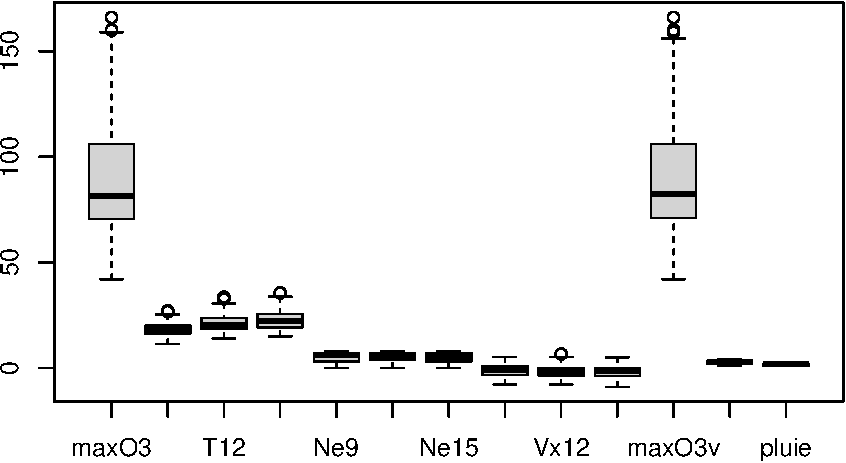
\includegraphics{TP-ML-Regression_files/figure-latex/unnamed-chunk-4-1.pdf}

\begin{Shaded}
\begin{Highlighting}[]
\FunctionTok{pairs}\NormalTok{(ozone)}
\end{Highlighting}
\end{Shaded}

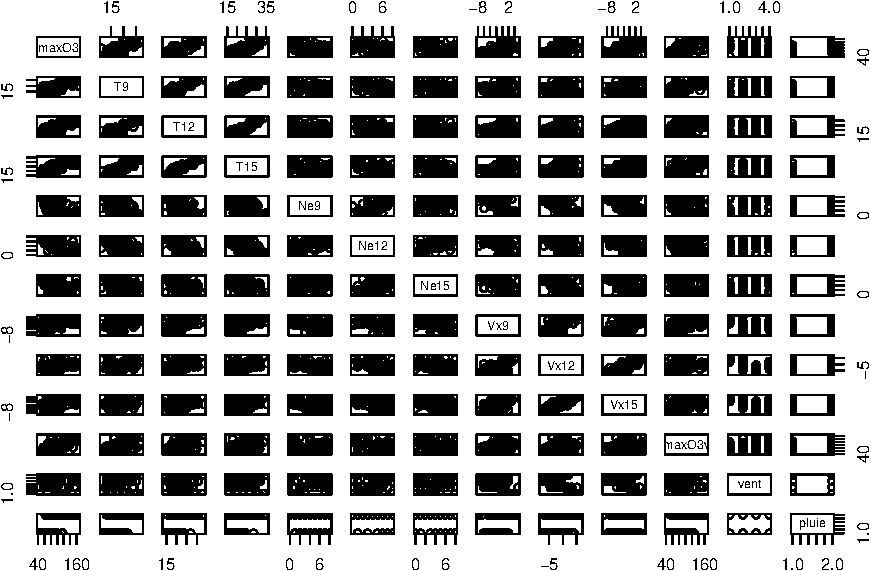
\includegraphics{TP-ML-Regression_files/figure-latex/unnamed-chunk-4-2.pdf}

\begin{Shaded}
\begin{Highlighting}[]
\FunctionTok{barplot}\NormalTok{(}\FunctionTok{cor}\NormalTok{(ozone[, }\DecValTok{1}\SpecialCharTok{:}\DecValTok{11}\NormalTok{]), }\AttributeTok{method =} \StringTok{"ellipse"}\NormalTok{)    }\CommentTok{\#?}
\end{Highlighting}
\end{Shaded}

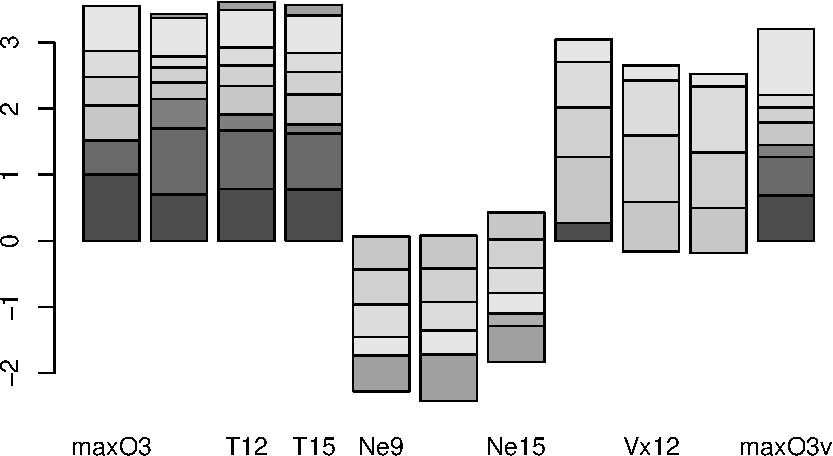
\includegraphics{TP-ML-Regression_files/figure-latex/unnamed-chunk-4-3.pdf}

\begin{Shaded}
\begin{Highlighting}[]
\NormalTok{corrplot}
\end{Highlighting}
\end{Shaded}

\begin{verbatim}
function (corr, method = c("circle", "square", "ellipse", "number", 
    "shade", "color", "pie"), type = c("full", "lower", "upper"), 
    col = NULL, col.lim = NULL, bg = "white", title = "", is.corr = TRUE, 
    add = FALSE, diag = TRUE, outline = FALSE, mar = c(0, 0, 
        0, 0), addgrid.col = NULL, addCoef.col = NULL, addCoefasPercent = FALSE, 
    order = c("original", "AOE", "FPC", "hclust", "alphabet"), 
    hclust.method = c("complete", "ward", "ward.D", "ward.D2", 
        "single", "average", "mcquitty", "median", "centroid"), 
    addrect = NULL, rect.col = "black", rect.lwd = 2, tl.pos = NULL, 
    tl.cex = 1, tl.col = "red", tl.offset = 0.4, tl.srt = 90, 
    cl.pos = NULL, cl.length = NULL, cl.cex = 0.8, cl.ratio = 0.15, 
    cl.align.text = "c", cl.offset = 0.5, number.cex = 1, number.font = 2, 
    number.digits = NULL, addshade = c("negative", "positive", 
        "all"), shade.lwd = 1, shade.col = "white", p.mat = NULL, 
    sig.level = 0.05, insig = c("pch", "p-value", "blank", "n", 
        "label_sig"), pch = 4, pch.col = "black", pch.cex = 3, 
    plotCI = c("n", "square", "circle", "rect"), lowCI.mat = NULL, 
    uppCI.mat = NULL, na.label = "?", na.label.col = "black", 
    win.asp = 1, ...) 
{
    method = match.arg(method)
    type = match.arg(type)
    order = match.arg(order)
    hclust.method = match.arg(hclust.method)
    addshade = match.arg(addshade)
    insig = match.arg(insig)
    plotCI = match.arg(plotCI)
    if (win.asp != 1 && !(method %in% c("circle", "square"))) {
        stop("Parameter 'win.asp' is supported only for circle and square methods.")
    }
    asp_rescale_factor = min(1, win.asp)/max(1, win.asp)
    stopifnot(asp_rescale_factor >= 0 && asp_rescale_factor <= 
        1)
    if (!is.matrix(corr) && !is.data.frame(corr)) {
        stop("Need a matrix or data frame!")
    }
    if (is.null(addgrid.col)) {
        addgrid.col = switch(method, color = NA, shade = NA, 
            "grey")
    }
    if (any(corr[!is.na(corr)] < col.lim[1]) || any(corr[!is.na(corr)] > 
        col.lim[2])) {
        stop("color limits should cover matrix")
    }
    if (is.null(col.lim)) {
        if (is.corr) {
            col.lim = c(-1, 1)
        }
        else {
            if (!diag) {
                diag(corr) = NA
            }
            col.lim = c(min(corr, na.rm = TRUE), max(corr, na.rm = TRUE))
        }
    }
    SpecialCorr = 0
    if (is.corr) {
        if (min(corr, na.rm = TRUE) < -1 - .Machine$double.eps^0.75 || 
            max(corr, na.rm = TRUE) > 1 + .Machine$double.eps^0.75) {
            stop("The matrix is not in [-1, 1]!")
        }
        SpecialCorr = 1
        if (col.lim[1] < -1 | col.lim[2] > 1) {
            stop("col.lim should be within the interval [-1, 1]")
        }
    }
    intercept = 0
    zoom = 1
    if (!is.corr) {
        c_max = max(corr, na.rm = TRUE)
        c_min = min(corr, na.rm = TRUE)
        if ((col.lim[1] > c_min) | (col.lim[2] < c_max)) {
            stop("Wrong color: matrix should be in col.lim interval!")
        }
        if (diff(col.lim)/(c_max - c_min) > 2) {
            warning("col.lim interval too wide, please set a suitable value")
        }
        if (c_max <= 0 | c_min >= 0) {
            intercept = -col.lim[1]
            zoom = 1/(diff(col.lim))
            if (col.lim[1] * col.lim[2] < 0) {
                warning("col.lim interval not suitable to the matrix")
            }
        }
        else {
            stopifnot(c_max * c_min < 0)
            stopifnot(c_min < 0 && c_max > 0)
            intercept = 0
            zoom = 1/max(abs(col.lim))
            SpecialCorr = 1
        }
        corr = (intercept + corr) * zoom
    }
    col.lim2 = (intercept + col.lim) * zoom
    int = intercept * zoom
    if (is.null(col) & is.corr) {
        col = COL2("RdBu", 200)
    }
    if (is.null(col) & !is.corr) {
        if (col.lim[1] * col.lim[2] < 0) {
            col = COL2("RdBu", 200)
        }
        else {
            col = COL1("YlOrBr", 200)
        }
    }
    n = nrow(corr)
    m = ncol(corr)
    min.nm = min(n, m)
    ord = 1:min.nm
    if (order != "original") {
        ord = corrMatOrder(corr, order = order, hclust.method = hclust.method)
        corr = corr[ord, ord]
    }
    if (is.null(rownames(corr))) {
        rownames(corr) = 1:n
    }
    if (is.null(colnames(corr))) {
        colnames(corr) = 1:m
    }
    apply_mat_filter = function(mat) {
        x = matrix(1:n * m, nrow = n, ncol = m)
        switch(type, upper = mat[row(x) > col(x)] <- Inf, lower = mat[row(x) < 
            col(x)] <- Inf)
        if (!diag) {
            diag(mat) = Inf
        }
        return(mat)
    }
    getPos.Dat = function(mat) {
        tmp = apply_mat_filter(mat)
        Dat = tmp[is.finite(tmp)]
        ind = which(is.finite(tmp), arr.ind = TRUE)
        Pos = ind
        Pos[, 1] = ind[, 2]
        Pos[, 2] = -ind[, 1] + 1 + n
        PosName = ind
        PosName[, 1] = colnames(mat)[ind[, 2]]
        PosName[, 2] = rownames(mat)[ind[, 1]]
        return(list(Pos, Dat, PosName))
    }
    getPos.NAs = function(mat) {
        tmp = apply_mat_filter(mat)
        ind = which(is.na(tmp), arr.ind = TRUE)
        Pos = ind
        Pos[, 1] = ind[, 2]
        Pos[, 2] = -ind[, 1] + 1 + n
        return(Pos)
    }
    testTemp = getPos.Dat(corr)
    Pos = getPos.Dat(corr)[[1]]
    PosName = getPos.Dat(corr)[[3]]
    if (any(is.na(corr)) && is.character(na.label)) {
        PosNA = getPos.NAs(corr)
    }
    else {
        PosNA = NULL
    }
    AllCoords = rbind(Pos, PosNA)
    n2 = max(AllCoords[, 2])
    n1 = min(AllCoords[, 2])
    nn = n2 - n1
    m2 = max(AllCoords[, 1])
    m1 = min(AllCoords[, 1])
    mm = max(1, m2 - m1)
    expand_expression = function(s) {
        ifelse(grepl("^[:=$]", s), parse(text = substring(s, 
            2)), s)
    }
    newrownames = sapply(rownames(corr)[(n + 1 - n2):(n + 1 - 
        n1)], expand_expression)
    newcolnames = sapply(colnames(corr)[m1:m2], expand_expression)
    DAT = getPos.Dat(corr)[[2]]
    len.DAT = length(DAT)
    rm(expand_expression)
    assign.color = function(dat = DAT, color = col, isSpecialCorr = SpecialCorr) {
        if (isSpecialCorr) {
            newcorr = (dat + 1)/2
        }
        else {
            newcorr = dat
        }
        newcorr[newcorr <= 0] = 0
        newcorr[newcorr >= 1] = 1 - 1e-16
        color[floor(newcorr * length(color)) + 1]
    }
    col.fill = assign.color()
    isFALSE = function(x) identical(x, FALSE)
    isTRUE = function(x) identical(x, TRUE)
    if (isFALSE(tl.pos)) {
        tl.pos = "n"
    }
    if (is.null(tl.pos) || isTRUE(tl.pos)) {
        tl.pos = switch(type, full = "lt", lower = "ld", upper = "td")
    }
    if (isFALSE(cl.pos)) {
        cl.pos = "n"
    }
    if (is.null(cl.pos) || isTRUE(cl.pos)) {
        cl.pos = switch(type, full = "r", lower = "b", upper = "r")
    }
    if (isFALSE(outline)) {
        col.border = col.fill
    }
    else if (isTRUE(outline)) {
        col.border = "black"
    }
    else if (is.character(outline)) {
        col.border = outline
    }
    else {
        stop("Unsupported value type for parameter outline")
    }
    oldpar = par(mar = mar, bg = par()$bg)
    on.exit(par(oldpar), add = TRUE)
    if (!add) {
        plot.new()
        xlabwidth = max(strwidth(newrownames, cex = tl.cex))
        ylabwidth = max(strwidth(newcolnames, cex = tl.cex))
        laboffset = strwidth("W", cex = tl.cex) * tl.offset
        for (i in 1:50) {
            xlim = c(m1 - 0.5 - laboffset - xlabwidth * (grepl("l", 
                tl.pos) | grepl("d", tl.pos)), m2 + 0.5 + mm * 
                cl.ratio * (cl.pos == "r") + xlabwidth * abs(cos(tl.srt * 
                pi/180)) * grepl("d", tl.pos))
            ylim = c(n1 - 0.5 - nn * cl.ratio * (cl.pos == "b") - 
                laboffset, n2 + 0.5 + laboffset + ylabwidth * 
                abs(sin(tl.srt * pi/180)) * grepl("t", tl.pos) + 
                ylabwidth * abs(sin(tl.srt * pi/180)) * (type == 
                  "lower") * grepl("d", tl.pos))
            plot.window(xlim, ylim, asp = 1, xaxs = "i", yaxs = "i")
            x.tmp = max(strwidth(newrownames, cex = tl.cex))
            y.tmp = max(strwidth(newcolnames, cex = tl.cex))
            laboffset.tmp = strwidth("W", cex = tl.cex) * tl.offset
            if (max(x.tmp - xlabwidth, y.tmp - ylabwidth, laboffset.tmp - 
                laboffset) < 0.001) {
                break
            }
            xlabwidth = x.tmp
            ylabwidth = y.tmp
            laboffset = laboffset.tmp
            if (i == 50) {
                warning(c("Not been able to calculate text margin, ", 
                  "please try again with a clean new empty window using ", 
                  "{plot.new(); dev.off()} or reduce tl.cex"))
            }
        }
        if (.Platform$OS.type == "windows") {
            grDevices::windows.options(width = 7, height = 7 * 
                diff(ylim)/diff(xlim))
        }
        xlim = xlim + diff(xlim) * 0.01 * c(-1, 1)
        ylim = ylim + diff(ylim) * 0.01 * c(-1, 1)
        plot.window(xlim = xlim, ylim = ylim, asp = win.asp, 
            xlab = "", ylab = "", xaxs = "i", yaxs = "i")
    }
    laboffset = strwidth("W", cex = tl.cex) * tl.offset
    symbols(Pos, add = TRUE, inches = FALSE, rectangles = matrix(1, 
        len.DAT, 2), bg = bg, fg = bg)
    if (method == "circle" && plotCI == "n") {
        symbols(Pos, add = TRUE, inches = FALSE, circles = asp_rescale_factor * 
            0.9 * abs(DAT)^0.5/2, fg = col.border, bg = col.fill)
    }
    if (method == "ellipse" && plotCI == "n") {
        ell.dat = function(rho, length = 99) {
            k = seq(0, 2 * pi, length = length)
            x = cos(k + acos(rho)/2)/2
            y = cos(k - acos(rho)/2)/2
            cbind(rbind(x, y), c(NA, NA))
        }
        ELL.dat = lapply(DAT, ell.dat)
        ELL.dat2 = 0.85 * matrix(unlist(ELL.dat), ncol = 2, byrow = TRUE)
        ELL.dat2 = ELL.dat2 + Pos[rep(1:length(DAT), each = 100), 
            ]
        polygon(ELL.dat2, border = col.border, col = col.fill)
    }
    if (is.null(number.digits)) {
        number.digits = switch(addCoefasPercent + 1, 2, 0)
    }
    stopifnot(number.digits%%1 == 0)
    stopifnot(number.digits >= 0)
    if (method == "number" && plotCI == "n") {
        x = (DAT - int) * ifelse(addCoefasPercent, 100, 1)/zoom
        text(Pos[, 1], Pos[, 2], font = number.font, col = col.fill, 
            labels = format(round(x, number.digits), nsmall = number.digits), 
            cex = number.cex)
    }
    NA_LABEL_MAX_CHARS = 2
    if (is.matrix(PosNA) && nrow(PosNA) > 0) {
        stopifnot(is.matrix(PosNA))
        if (na.label == "square") {
            symbols(PosNA, add = TRUE, inches = FALSE, squares = rep(1, 
                nrow(PosNA)), bg = na.label.col, fg = na.label.col)
        }
        else if (nchar(na.label) %in% 1:NA_LABEL_MAX_CHARS) {
            symbols(PosNA, add = TRUE, inches = FALSE, squares = rep(1, 
                nrow(PosNA)), fg = bg, bg = bg)
            text(PosNA[, 1], PosNA[, 2], font = number.font, 
                col = na.label.col, labels = na.label, cex = number.cex, 
                ...)
        }
        else {
            stop(paste("Maximum number of characters for NA label is:", 
                NA_LABEL_MAX_CHARS))
        }
    }
    if (method == "pie" && plotCI == "n") {
        symbols(Pos, add = TRUE, inches = FALSE, circles = rep(0.5, 
            len.DAT) * 0.85, fg = col.border)
        pie.dat = function(theta, length = 100) {
            k = seq(pi/2, pi/2 - theta, length = 0.5 * length * 
                abs(theta)/pi)
            x = c(0, cos(k)/2, 0)
            y = c(0, sin(k)/2, 0)
            cbind(rbind(x, y), c(NA, NA))
        }
        PIE.dat = lapply(DAT * 2 * pi, pie.dat)
        len.pie = unlist(lapply(PIE.dat, length))/2
        PIE.dat2 = 0.85 * matrix(unlist(PIE.dat), ncol = 2, byrow = TRUE)
        PIE.dat2 = PIE.dat2 + Pos[rep(1:length(DAT), len.pie), 
            ]
        polygon(PIE.dat2, border = "black", col = col.fill)
    }
    if (method == "shade" && plotCI == "n") {
        symbols(Pos, add = TRUE, inches = FALSE, squares = rep(1, 
            len.DAT), bg = col.fill, fg = addgrid.col)
        shade.dat = function(w) {
            x = w[1]
            y = w[2]
            rho = w[3]
            x1 = x - 0.5
            x2 = x + 0.5
            y1 = y - 0.5
            y2 = y + 0.5
            dat = NA
            if ((addshade == "positive" || addshade == "all") && 
                rho > 0) {
                dat = cbind(c(x1, x1, x), c(y, y1, y1), c(x, 
                  x2, x2), c(y2, y2, y))
            }
            if ((addshade == "negative" || addshade == "all") && 
                rho < 0) {
                dat = cbind(c(x1, x1, x), c(y, y2, y2), c(x, 
                  x2, x2), c(y1, y1, y))
            }
            return(t(dat))
        }
        pos_corr = rbind(cbind(Pos, DAT))
        pos_corr2 = split(pos_corr, 1:nrow(pos_corr))
        SHADE.dat = matrix(na.omit(unlist(lapply(pos_corr2, shade.dat))), 
            byrow = TRUE, ncol = 4)
        segments(SHADE.dat[, 1], SHADE.dat[, 2], SHADE.dat[, 
            3], SHADE.dat[, 4], col = shade.col, lwd = shade.lwd)
    }
    if (method == "square" && plotCI == "n") {
        draw_method_square(Pos, DAT, asp_rescale_factor, col.border, 
            col.fill)
    }
    if (method == "color" && plotCI == "n") {
        draw_method_color(Pos, col.border, col.fill)
    }
    draw_grid(AllCoords, addgrid.col)
    if (plotCI != "n") {
        if (is.null(lowCI.mat) || is.null(uppCI.mat)) {
            stop("Need lowCI.mat and uppCI.mat!")
        }
        if (order != "original") {
            lowCI.mat = lowCI.mat[ord, ord]
            uppCI.mat = uppCI.mat[ord, ord]
        }
        pos.lowNew = getPos.Dat(lowCI.mat)[[1]]
        lowNew = getPos.Dat(lowCI.mat)[[2]]
        pos.uppNew = getPos.Dat(uppCI.mat)[[1]]
        uppNew = getPos.Dat(uppCI.mat)[[2]]
        k1 = (abs(uppNew) > abs(lowNew))
        bigabs = uppNew
        bigabs[which(!k1)] = lowNew[!k1]
        smallabs = lowNew
        smallabs[which(!k1)] = uppNew[!k1]
        sig = sign(uppNew * lowNew)
        color_bigabs = col[ceiling((bigabs + 1) * length(col)/2)]
        color_smallabs = col[ceiling((smallabs + 1) * length(col)/2)]
        if (plotCI == "circle") {
            symbols(pos.uppNew[, 1], pos.uppNew[, 2], add = TRUE, 
                inches = FALSE, circles = 0.95 * abs(bigabs)^0.5/2, 
                bg = ifelse(sig > 0, col.fill, color_bigabs), 
                fg = ifelse(sig > 0, col.fill, color_bigabs))
            symbols(pos.lowNew[, 1], pos.lowNew[, 2], add = TRUE, 
                inches = FALSE, circles = 0.95 * abs(smallabs)^0.5/2, 
                bg = ifelse(sig > 0, bg, color_smallabs), fg = ifelse(sig > 
                  0, col.fill, color_smallabs))
        }
        if (plotCI == "square") {
            symbols(pos.uppNew[, 1], pos.uppNew[, 2], add = TRUE, 
                inches = FALSE, squares = abs(bigabs)^0.5, bg = ifelse(sig > 
                  0, col.fill, color_bigabs), fg = ifelse(sig > 
                  0, col.fill, color_bigabs))
            symbols(pos.lowNew[, 1], pos.lowNew[, 2], add = TRUE, 
                inches = FALSE, squares = abs(smallabs)^0.5, 
                bg = ifelse(sig > 0, bg, color_smallabs), fg = ifelse(sig > 
                  0, col.fill, color_smallabs))
        }
        if (plotCI == "rect") {
            rect.width = 0.25
            rect(pos.uppNew[, 1] - rect.width, pos.uppNew[, 2] + 
                smallabs/2, pos.uppNew[, 1] + rect.width, pos.uppNew[, 
                2] + bigabs/2, col = col.fill, border = col.fill)
            segments(pos.lowNew[, 1] - rect.width, pos.lowNew[, 
                2] + DAT/2, pos.lowNew[, 1] + rect.width, pos.lowNew[, 
                2] + DAT/2, col = "black", lwd = 1)
            segments(pos.uppNew[, 1] - rect.width, pos.uppNew[, 
                2] + uppNew/2, pos.uppNew[, 1] + rect.width, 
                pos.uppNew[, 2] + uppNew/2, col = "black", lwd = 1)
            segments(pos.lowNew[, 1] - rect.width, pos.lowNew[, 
                2] + lowNew/2, pos.lowNew[, 1] + rect.width, 
                pos.lowNew[, 2] + lowNew/2, col = "black", lwd = 1)
            segments(pos.lowNew[, 1] - 0.5, pos.lowNew[, 2], 
                pos.lowNew[, 1] + 0.5, pos.lowNew[, 2], col = "grey70", 
                lty = 3)
        }
    }
    if (!is.null(addCoef.col) && method != "number") {
        text(Pos[, 1], Pos[, 2], col = addCoef.col, labels = round((DAT - 
            int) * ifelse(addCoefasPercent, 100, 1)/zoom, number.digits), 
            cex = number.cex, font = number.font)
    }
    if (!is.null(p.mat) && insig != "n") {
        if (order != "original") {
            p.mat = p.mat[ord, ord]
        }
        if (!is.null(rownames(p.mat)) | !is.null(rownames(p.mat))) {
            if (!all(colnames(p.mat) == colnames(corr)) | !all(rownames(p.mat) == 
                rownames(corr))) {
                warning("p.mat and corr may be not paired, their rownames and colnames are not totally same!")
            }
        }
        pos.pNew = getPos.Dat(p.mat)[[1]]
        pNew = getPos.Dat(p.mat)[[2]]
        if (insig == "label_sig") {
            if (!is.character(pch)) 
                pch = "*"
            place_points = function(sig.locs, point) {
                text(pos.pNew[, 1][sig.locs], pos.pNew[, 2][sig.locs], 
                  labels = point, col = pch.col, cex = pch.cex, 
                  lwd = 2)
            }
            if (length(sig.level) == 1) {
                place_points(sig.locs = which(pNew < sig.level), 
                  point = pch)
            }
            else {
                l = length(sig.level)
                for (i in seq_along(sig.level)) {
                  iter = l + 1 - i
                  pchTmp = paste(rep(pch, i), collapse = "")
                  if (i == length(sig.level)) {
                    locs = which(pNew < sig.level[iter])
                    if (length(locs)) {
                      place_points(sig.locs = locs, point = pchTmp)
                    }
                  }
                  else {
                    locs = which(pNew < sig.level[iter] & pNew > 
                      sig.level[iter - 1])
                    if (length(locs)) {
                      place_points(sig.locs = locs, point = pchTmp)
                    }
                  }
                }
            }
        }
        else {
            ind.p = which(pNew > sig.level)
            p_inSig = length(ind.p) > 0
            if (insig == "pch" && p_inSig) {
                points(pos.pNew[, 1][ind.p], pos.pNew[, 2][ind.p], 
                  pch = pch, col = pch.col, cex = pch.cex, lwd = 2)
            }
            if (insig == "p-value" && p_inSig) {
                text(pos.pNew[, 1][ind.p], pos.pNew[, 2][ind.p], 
                  round(pNew[ind.p], number.digits), col = pch.col)
            }
            if (insig == "blank" && p_inSig) {
                symbols(pos.pNew[, 1][ind.p], pos.pNew[, 2][ind.p], 
                  inches = FALSE, squares = rep(1, length(pos.pNew[, 
                    1][ind.p])), fg = addgrid.col, bg = bg, add = TRUE)
            }
        }
    }
    if (cl.pos != "n") {
        colRange = assign.color(dat = col.lim2)
        ind1 = which(col == colRange[1])
        ind2 = which(col == colRange[2])
        colbar = col[ind1:ind2]
        if (is.null(cl.length)) {
            cl.length = ifelse(length(colbar) > 20, 11, length(colbar) + 
                1)
        }
        labels = seq(col.lim[1], col.lim[2], length = cl.length)
        if (cl.pos == "r") {
            vertical = TRUE
            xlim = c(m2 + 0.5 + mm * 0.02, m2 + 0.5 + mm * cl.ratio)
            ylim = c(n1 - 0.5, n2 + 0.5)
        }
        if (cl.pos == "b") {
            vertical = FALSE
            xlim = c(m1 - 0.5, m2 + 0.5)
            ylim = c(n1 - 0.5 - nn * cl.ratio, n1 - 0.5 - nn * 
                0.02)
        }
        colorlegend(colbar = colbar, labels = round(labels, 2), 
            offset = cl.offset, ratio.colbar = 0.3, cex = cl.cex, 
            xlim = xlim, ylim = ylim, vertical = vertical, align = cl.align.text)
    }
    if (tl.pos != "n") {
        pos.xlabel = cbind(m1:m2, n2 + 0.5 + laboffset)
        pos.ylabel = cbind(m1 - 0.5, n2:n1)
        if (tl.pos == "td") {
            if (type != "upper") {
                stop("type should be 'upper' if tl.pos is 'dt'.")
            }
            pos.ylabel = cbind(m1:(m1 + nn) - 0.5, n2:n1)
        }
        if (tl.pos == "ld") {
            if (type != "lower") {
                stop("type should be 'lower' if tl.pos is 'ld'.")
            }
            pos.xlabel = cbind(m1:m2, n2:(n2 - mm) + 0.5 + laboffset)
        }
        if (tl.pos == "d") {
            pos.ylabel = cbind(m1:(m1 + nn) - 0.5, n2:n1)
            pos.ylabel = pos.ylabel[1:min(n, m), ]
            symbols(pos.ylabel[, 1] + 0.5, pos.ylabel[, 2], add = TRUE, 
                bg = bg, fg = addgrid.col, inches = FALSE, squares = rep(1, 
                  length(pos.ylabel[, 1])))
            text(pos.ylabel[, 1] + 0.5, pos.ylabel[, 2], newcolnames[1:min(n, 
                m)], col = tl.col, cex = tl.cex, ...)
        }
        else {
            if (tl.pos != "l") {
                text(pos.xlabel[, 1], pos.xlabel[, 2], newcolnames, 
                  srt = tl.srt, adj = ifelse(tl.srt == 0, c(0.5, 
                    0), c(0, 0)), col = tl.col, cex = tl.cex, 
                  offset = tl.offset, ...)
            }
            text(pos.ylabel[, 1], pos.ylabel[, 2], newrownames, 
                col = tl.col, cex = tl.cex, pos = 2, offset = tl.offset, 
                ...)
        }
    }
    title(title, ...)
    if (type == "full" && plotCI == "n" && !is.null(addgrid.col)) {
        rect(m1 - 0.5, n1 - 0.5, m2 + 0.5, n2 + 0.5, border = addgrid.col)
    }
    if (!is.null(addrect) && order == "hclust" && type == "full") {
        corrRect.hclust(corr, k = addrect, method = hclust.method, 
            col = rect.col, lwd = rect.lwd)
    }
    corrPos = data.frame(PosName, Pos, DAT)
    colnames(corrPos) = c("xName", "yName", "x", "y", "corr")
    if (!is.null(p.mat)) {
        corrPos = cbind(corrPos, pNew)
        colnames(corrPos)[6] = c("p.value")
    }
    corrPos = corrPos[order(corrPos[, 3], -corrPos[, 4]), ]
    rownames(corrPos) = NULL
    res = list(corr = corr, corrPos = corrPos, arg = list(type = type))
    invisible(res)
}
<bytecode: 0x5572d0693388>
<environment: namespace:corrplot>
\end{verbatim}

\begin{Shaded}
\begin{Highlighting}[]
\CommentTok{\# On remarque alors que les variables semblent pour certains blocs très corrélés. On verra donc si on peut peut{-}être exprimer un sous{-}modèle (ne prenant par exemple en variables qu\textquotesingle{}un seul T\_i, Ne\_i, Vx\_i)}
\end{Highlighting}
\end{Shaded}

\hypertarget{ruxe9gression-linuxe9aire-simple}{%
\section{Régression linéaire
simple}\label{ruxe9gression-linuxe9aire-simple}}

Dans cette section, nous souhaitons expliquer la concentration d'ozone
maximale de la journée (maxO3) en fonction de la température à 12h
(T12).

\begin{enumerate}
\def\labelenumi{\arabic{enumi}.}
\tightlist
\item
  Représentez le nuage de points \((x_i,y_i)\) à l'aide de la fonction
  \texttt{plot()} (ou \texttt{geom\_point()} de \emph{ggplot2}).
\end{enumerate}

\begin{Shaded}
\begin{Highlighting}[]
\CommentTok{\# A completer}
\FunctionTok{plot}\NormalTok{(ozone}\SpecialCharTok{$}\NormalTok{T12, ozone}\SpecialCharTok{$}\NormalTok{maxO3)}
\end{Highlighting}
\end{Shaded}

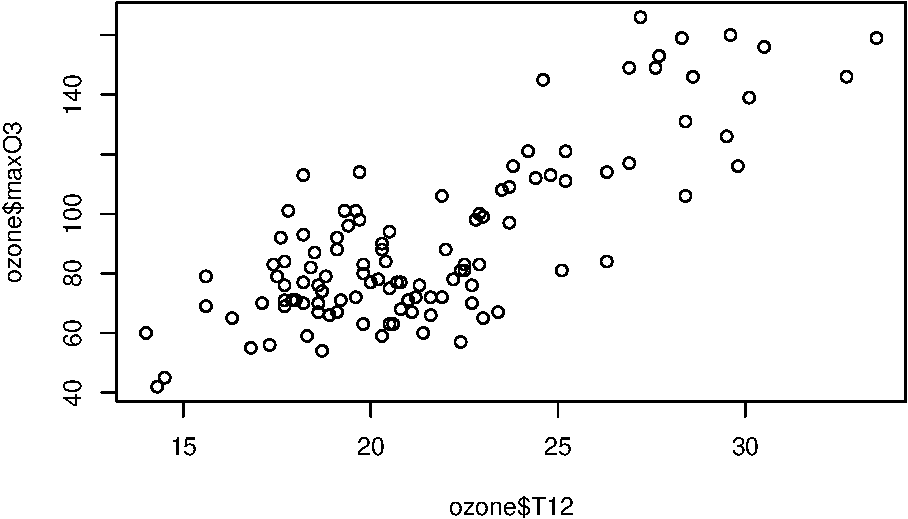
\includegraphics{TP-ML-Regression_files/figure-latex/unnamed-chunk-6-1.pdf}

\begin{Shaded}
\begin{Highlighting}[]
\CommentTok{\#ggplot(ozone, aes(x = T12, y = max)) \# A FINIR}
\end{Highlighting}
\end{Shaded}

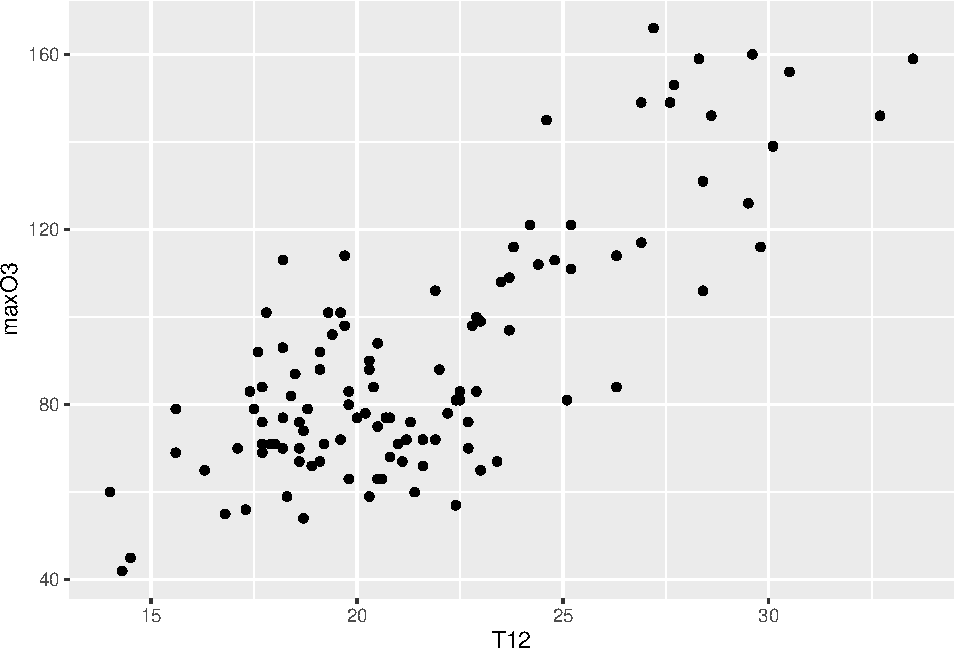
\includegraphics{TP-ML-Regression_files/figure-latex/unnamed-chunk-7-1.pdf}

Question : Pensez-vous que l'ajustement d'un modèle de régression
linéaire \(y_i = \theta_0+\theta_1 x_i +\varepsilon_i\) est justifié
graphiquement?

Réponse : \ldots{} On remarque que les points semblent globalement
distribués autour d'une droite, que l'on peut effectivement modéliser
par \(y_i = \theta_0+\theta_1 x_i +\varepsilon_i\).

\begin{enumerate}
\def\labelenumi{\arabic{enumi}.}
\setcounter{enumi}{1}
\tightlist
\item
  Effectuez la régression linéaire à l'aide de la fonction \texttt{lm()}
  et exploitez les résultats.
\end{enumerate}

\begin{Shaded}
\begin{Highlighting}[]
\NormalTok{reg.simple }\OtherTok{=} \FunctionTok{lm}\NormalTok{(maxO3 }\SpecialCharTok{\textasciitilde{}}\NormalTok{ T12, }\AttributeTok{data =}\NormalTok{ ozone)  }\CommentTok{\# COMPLETE}
\FunctionTok{summary}\NormalTok{(reg.simple)}
\end{Highlighting}
\end{Shaded}

\begin{verbatim}

Call:
lm(formula = maxO3 ~ T12, data = ozone)

Residuals:
    Min      1Q  Median      3Q     Max 
-38.079 -12.735   0.257  11.003  44.671 

Coefficients:
            Estimate Std. Error t value Pr(>|t|)    
(Intercept) -27.4196     9.0335  -3.035    0.003 ** 
T12           5.4687     0.4125  13.258   <2e-16 ***
---
Signif. codes:  0 '***' 0.001 '**' 0.01 '*' 0.05 '.' 0.1 ' ' 1

Residual standard error: 17.57 on 110 degrees of freedom
Multiple R-squared:  0.6151,    Adjusted R-squared:  0.6116 
F-statistic: 175.8 on 1 and 110 DF,  p-value: < 2.2e-16
\end{verbatim}

Interprétation : \ldots.. 17.57 est la \(\sigma^{chapeau}^2\),
\(110 = n - 2\) (\(k = 2\)) On récupère bien de l'information au travers
de T12, (on rejette \(\mathcal{H_0}\)).

Que contiennent les sorties suivantes :

\begin{Shaded}
\begin{Highlighting}[]
\NormalTok{reg.simple}\SpecialCharTok{$}\NormalTok{coefficients  }
\end{Highlighting}
\end{Shaded}

\begin{verbatim}
(Intercept)         T12 
 -27.419636    5.468685 
\end{verbatim}

\begin{Shaded}
\begin{Highlighting}[]
\NormalTok{reg.simple}\SpecialCharTok{$}\NormalTok{residuals}
\end{Highlighting}
\end{Shaded}

\begin{verbatim}
   20010601    20010602    20010603    20010604    20010605    20010606 
 13.2489658   8.7958343  23.1707822  33.6865440   9.3115961  -0.8603245 
   20010607    20010610    20010611    20010612    20010613    20010614 
 21.1081519  10.7176507  21.2334124  13.6554373  22.8740179   6.4053330 
   20010615    20010616    20010617    20010618    20010620    20010621 
 -7.7665876  -2.1104287  15.2645192  10.9677549  37.8899881 -14.0789052 
   20010622    20010623    20010624    20010625    20010626    20010627 
 16.0774621  17.0152486  10.6087772  -5.4063593   6.9055415 -14.8132476 
   20010628    20010629    20010630    20010701    20010702    20010703 
-38.0789052 -28.8443543 -33.5475900 -26.7195106 -21.8910144   1.8122213 
   20010704    20010705    20010706    20010707    20010708    20010709 
  3.6083603  20.8895713  -5.1881955  40.8895713 -16.5164833  -4.8914312 
   20010710    20010711    20010712    20010713    20010714    20010715 
 -8.7821409 -16.4227464 -11.1886124  -6.8762947  -7.2979027 -10.0322451 
   20010716    20010717    20010718    20010719    20010720    20010721 
 -0.1415354 -21.6884039  11.1081519  14.9677549   4.4053330 -24.7039573 
   20010722    20010723    20010724    20010725    20010726    20010727 
-20.3445627 -14.6257737 -12.6257737  29.3120129  28.9370650  31.6558541 
   20010728    20010729    20010730    20010731    20010801    20010802 
 25.4839335  25.5465638  16.6247474 -32.4067762  -7.9065677  13.2649360 
   20010803    20010804    20010805    20010806    20010807    20010808 
  4.8895713 -22.2352724 -20.8447712 -33.3601161 -18.7039573 -29.6102203 
   20010809    20010810    20010811    20010812    20010813    20010814 
  3.9051246  -4.9540615   0.7336209   0.6087772  -9.6884039 -19.5471732 
   20010815    20010819    20010820 
  6.8118045 -20.9696149 -13.0633518 
 [ reached getOption("max.print") -- omitted 37 entries ]
\end{verbatim}

Réponse : \ldots{} Première commande : \(\hat{\theta}^{obs}\) Deuxième
commande : \(\hat{\varepsilon}_{i}^{obs}\) On peut obtenur les
\(\hat{Y}_{i}^{obs}\) avec :

\begin{Shaded}
\begin{Highlighting}[]
\NormalTok{reg.simple}\SpecialCharTok{$}\NormalTok{fitted.values}
\end{Highlighting}
\end{Shaded}

\begin{verbatim}
 20010601  20010602  20010603  20010604  20010605  20010606  20010607  20010610 
 73.75103  73.20417  68.82922  80.31346  84.68840  80.86032  57.89185  68.28235 
 20010611  20010612  20010613  20010614  20010615  20010616  20010617  20010618 
 79.76659  92.34456  78.12598  83.59467  79.76659  72.11043  67.73548  77.03225 
 20010620  20010621  20010622  20010623  20010624  20010625  20010626  20010627 
107.11001  95.07891 104.92254 128.98475 110.39122 151.40636 101.09446  97.81325 
 20010628  20010629  20010630  20010701  20010702  20010703  20010704  20010705 
 95.07891 109.84435 100.54759  96.71951 127.89101 137.18778  75.39164  72.11043 
 20010706  20010707  20010708  20010709  20010710  20010711  20010712  20010713 
102.18820  72.11043  88.51648  92.89143  85.78214  87.42275  67.18861  51.87629 
 20010714  20010715  20010716  20010717  20010718  20010719  20010720  20010721 
 74.29790  77.03225  84.14154  84.68840  57.89185  77.03225  83.59467  90.70396 
 20010722  20010723  20010724  20010725  20010726  20010727  20010728  20010729 
 92.34456  95.62577  95.62577 119.68799 124.06293 127.34415 123.51607 134.45344 
 20010730  20010731  20010801  20010802  20010803  20010804  20010805  20010806 
139.37525 116.40678 133.90657 102.73506  72.11043  85.23527  74.84477  98.36012 
 20010807  20010808  20010809  20010810  20010811  20010812  20010813  20010814 
 90.70396  89.61022  66.09488  81.95406  97.26638 110.39122  84.68840 135.54717 
 20010815  20010819  20010820 
102.18820  87.96961  89.06335 
 [ reached getOption("max.print") -- omitted 37 entries ]
\end{verbatim}

\begin{enumerate}
\def\labelenumi{\arabic{enumi}.}
\setcounter{enumi}{2}
\tightlist
\item
  A l'aide des commandes suivantes, tracez l'estimation de la droite de
  régression sur le nuage de points ainsi qu'un intervalle de confiance
  à \(95\%\) de celle-ci :
\end{enumerate}

\begin{Shaded}
\begin{Highlighting}[]
\FunctionTok{ggplot}\NormalTok{(ozone, }\FunctionTok{aes}\NormalTok{(T12, maxO3))}\SpecialCharTok{+}
    \FunctionTok{geom\_point}\NormalTok{() }\SpecialCharTok{+}
    \FunctionTok{geom\_smooth}\NormalTok{(}\AttributeTok{method=}\NormalTok{lm, }\AttributeTok{se=}\ConstantTok{TRUE}\NormalTok{)}\SpecialCharTok{+}
    \FunctionTok{xlab}\NormalTok{(}\StringTok{"T12"}\NormalTok{)}\SpecialCharTok{+}  \FunctionTok{ylab}\NormalTok{(}\StringTok{"maxO3"}\NormalTok{)}
\end{Highlighting}
\end{Shaded}

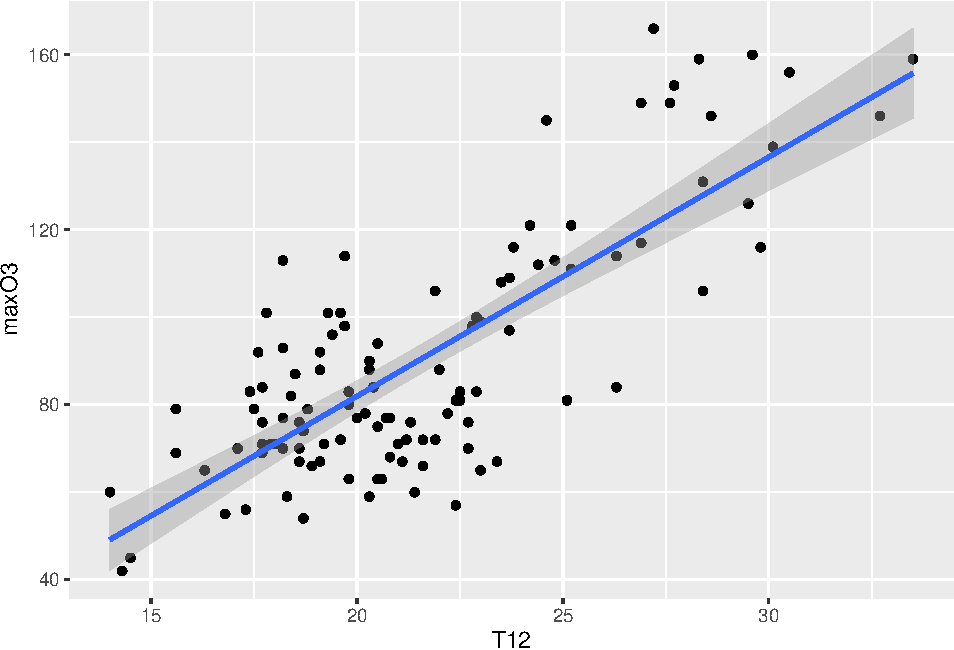
\includegraphics{TP-ML-Regression_files/figure-latex/unnamed-chunk-11-1.pdf}

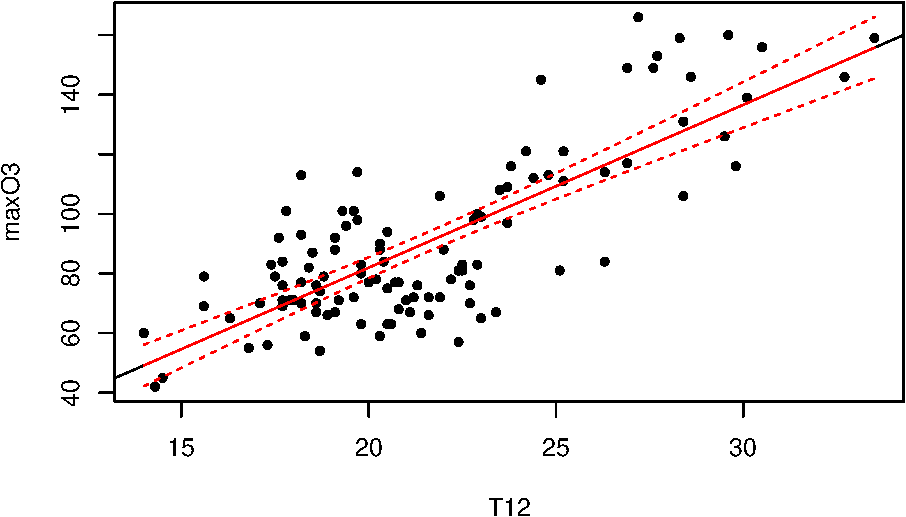
\includegraphics{TP-ML-Regression_files/figure-latex/unnamed-chunk-12-1.pdf}
REM : on a
\(IC_{1 - \alpha = 0,95}(X_0\theta) = [X_0\hat{\theta} + ou - t_{0,975}\sqrt{\hat{\sigma}^{2}X_0(X'X)^{-1}X_0'}]\)

Ce graphique permet visuellement de vérifier l'ajustement des données au
modèle de régression linéaire. Que remarquez-vous?

\begin{enumerate}
\def\labelenumi{\arabic{enumi}.}
\setcounter{enumi}{3}
\tightlist
\item
  A l'aide de la commande suivante, étudiez les résidus
\end{enumerate}

\begin{Shaded}
\begin{Highlighting}[]
\FunctionTok{autoplot}\NormalTok{(reg.simple,}\AttributeTok{which=}\FunctionTok{c}\NormalTok{(}\DecValTok{1}\NormalTok{,}\DecValTok{2}\NormalTok{,}\DecValTok{4}\NormalTok{),}\AttributeTok{label.size=}\DecValTok{2}\NormalTok{)     }
\end{Highlighting}
\end{Shaded}

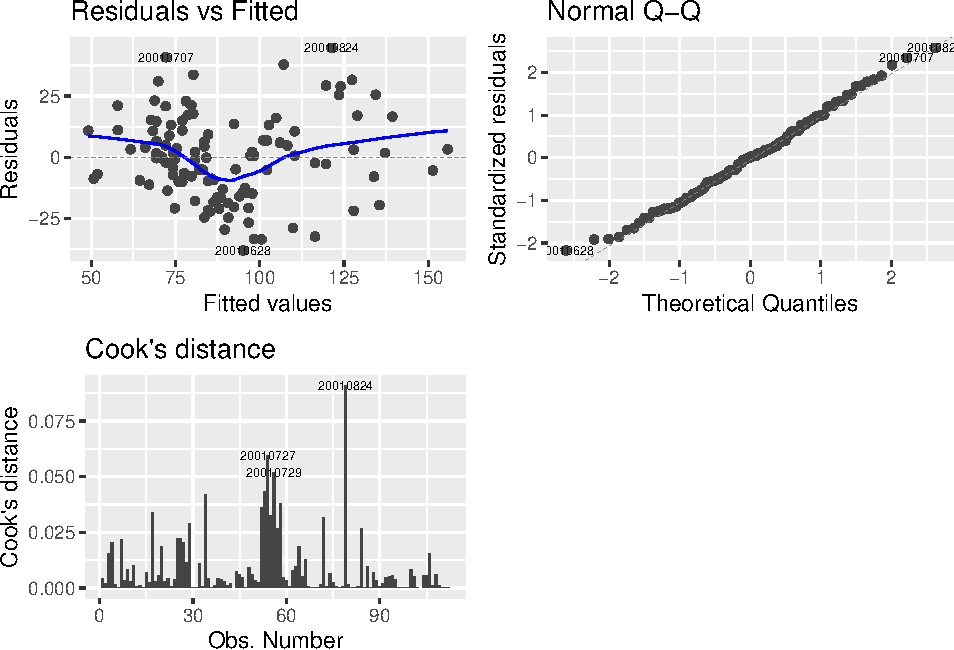
\includegraphics{TP-ML-Regression_files/figure-latex/unnamed-chunk-13-1.pdf}

On prendra soin de comprendre les différents graphiques obtenus.

REM : Sur le premier graphe qui représente les
\(\varepsilon^{chapeau}_i\) en fonction de ??, on observe que les
erreurs sont globalement distribuées autour de 0. On voit aussi les
numéro des individus sortant un peu trop de la tendance. Une idée
pourrait donc de les supprimer et de refaire l'observation.

Le deuxième graphe représentes les quantiles standardisés en fonctions
des quantiles théoriques. L'allure linéaire de ce graphe nous permet de
dire que le modèle gaussien semblent donc convenir.

\begin{enumerate}
\def\labelenumi{\arabic{enumi}.}
\setcounter{enumi}{4}
\tightlist
\item
  On s'intéresse maintenant à la qualité de prédiction du modèle. On va
  donc tracer un intervalle de confiance des prédictions à \(95\%\) avec
  les commandes suivantes. Commentez.
\end{enumerate}

\begin{Shaded}
\begin{Highlighting}[]
\NormalTok{temp\_var }\OtherTok{=} \FunctionTok{predict}\NormalTok{(reg.simple, }
                  \AttributeTok{interval=}\StringTok{"prediction"}\NormalTok{)}
\NormalTok{new\_df }\OtherTok{=} \FunctionTok{cbind}\NormalTok{(ozone, temp\_var)}
\FunctionTok{ggplot}\NormalTok{(new\_df, }\FunctionTok{aes}\NormalTok{(T12, maxO3))}\SpecialCharTok{+}
    \FunctionTok{geom\_point}\NormalTok{() }\SpecialCharTok{+}
    \FunctionTok{geom\_line}\NormalTok{(}\FunctionTok{aes}\NormalTok{(}\AttributeTok{y=}\NormalTok{lwr), }\AttributeTok{color =} \StringTok{"red"}\NormalTok{, }
                       \AttributeTok{linetype =} \StringTok{"dashed"}\NormalTok{)}\SpecialCharTok{+}
    \FunctionTok{geom\_line}\NormalTok{(}\FunctionTok{aes}\NormalTok{(}\AttributeTok{y=}\NormalTok{upr), }\AttributeTok{color =} \StringTok{"red"}\NormalTok{, }
                       \AttributeTok{linetype =} \StringTok{"dashed"}\NormalTok{)}\SpecialCharTok{+}
    \FunctionTok{geom\_smooth}\NormalTok{(}\AttributeTok{method=}\NormalTok{lm, }\AttributeTok{se=}\ConstantTok{TRUE}\NormalTok{)}\SpecialCharTok{+}
    \FunctionTok{xlab}\NormalTok{(}\StringTok{"T12"}\NormalTok{)}\SpecialCharTok{+}  
    \FunctionTok{ylab}\NormalTok{(}\StringTok{"maxO3"}\NormalTok{)}
\end{Highlighting}
\end{Shaded}

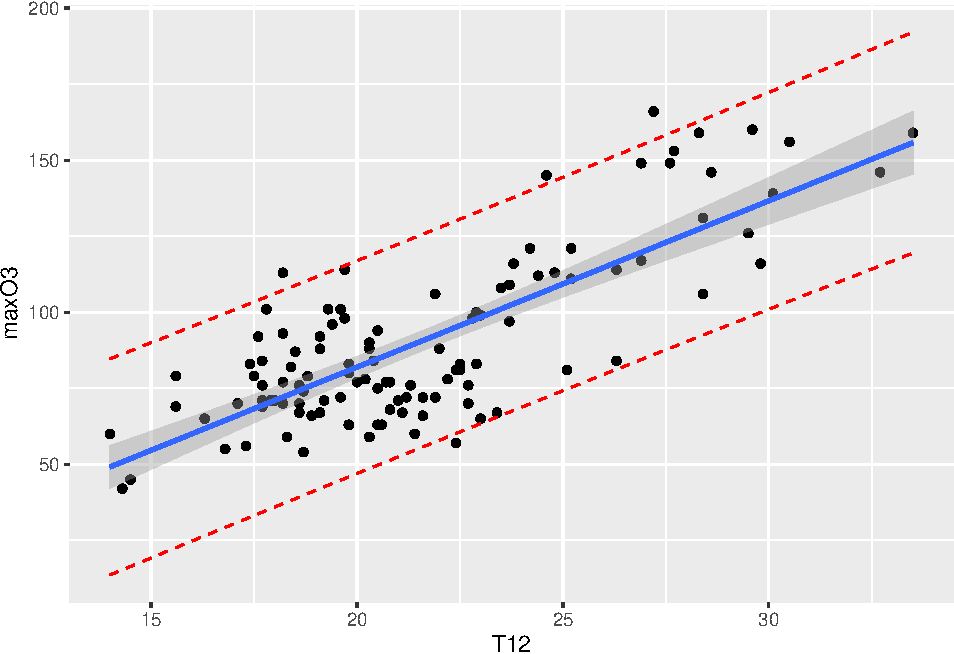
\includegraphics{TP-ML-Regression_files/figure-latex/unnamed-chunk-14-1.pdf}

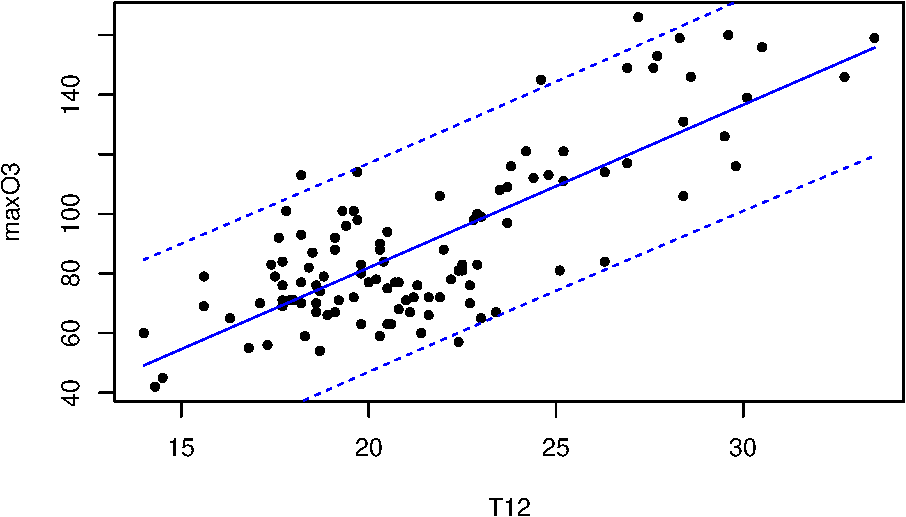
\includegraphics{TP-ML-Regression_files/figure-latex/unnamed-chunk-15-1.pdf}
REM : Commentaires : On a :
\(IC_{1 - \alpha = 0,95}(X_0\theta) = [X_0\hat{\theta} + ou - t_{0,975}\sqrt{\sigma^{2}(1 + X_0(X'X)^{-1}X_0')}]\)

\begin{enumerate}
\def\labelenumi{\arabic{enumi}.}
\setcounter{enumi}{5}
\tightlist
\item
  On va maintenant s'intéresser à la construction d'intervalles de
  confiance pour \(\theta_0\) et \(\theta_1\) à \(95\%\).\\
  A l'aide de la fonction \texttt{confint()}, construisez un intervalle
  de confiance pour chaque paramètre séparément.
\end{enumerate}

Ici, A COMPLETER

\begin{Shaded}
\begin{Highlighting}[]
\CommentTok{\# A COMPLETER}
\NormalTok{IC }\OtherTok{=} \FunctionTok{confint}\NormalTok{(reg.simple)}
\FunctionTok{print}\NormalTok{(IC)}
\end{Highlighting}
\end{Shaded}

\begin{verbatim}
                 2.5 %    97.5 %
(Intercept) -45.321901 -9.517371
T12           4.651219  6.286151
\end{verbatim}

Pour tenir compte de la dépendance entre \(\theta_0\) et \(\theta_1\),
on peut aussi construire une région de confiance pour le vecteur
\(\theta=(\theta_0,\theta_1)'\) grâce aux commandes suivantes. Comparez
les résultats.

Ici, il faut suivre la construction d'une région de confiance pour \$
C\theta\$ avec \(C=I_2\) ici.

\begin{Shaded}
\begin{Highlighting}[]
\NormalTok{df1 }\OtherTok{=} \FunctionTok{as.data.frame}\NormalTok{(}
             \FunctionTok{rbind}\NormalTok{(}\FunctionTok{coefficients}\NormalTok{(reg.simple),}
             \FunctionTok{ellipse}\NormalTok{(reg.simple,}\AttributeTok{level=}\FloatTok{0.95}\NormalTok{)))}
\FunctionTok{colnames}\NormalTok{(df1) }\OtherTok{=} \FunctionTok{c}\NormalTok{(}\StringTok{"intp"}\NormalTok{, }\StringTok{"slope"}\NormalTok{)}
\FunctionTok{ggplot}\NormalTok{(}\AttributeTok{data=}\NormalTok{df1[}\SpecialCharTok{{-}}\DecValTok{1}\NormalTok{,],}\FunctionTok{aes}\NormalTok{(}\AttributeTok{x=}\NormalTok{intp, }\AttributeTok{y=}\NormalTok{slope))}\SpecialCharTok{+}
  \FunctionTok{geom\_path}\NormalTok{()}\SpecialCharTok{+}
  \FunctionTok{annotate}\NormalTok{(}\StringTok{"rect"}\NormalTok{,}\AttributeTok{xmin=}\NormalTok{IC[}\DecValTok{1}\NormalTok{,}\DecValTok{1}\NormalTok{],}\AttributeTok{xmax=}\NormalTok{IC[}\DecValTok{1}\NormalTok{,}\DecValTok{2}\NormalTok{],}
  \AttributeTok{ymin=}\NormalTok{IC[}\DecValTok{2}\NormalTok{,}\DecValTok{1}\NormalTok{],}\AttributeTok{ymax=}\NormalTok{IC[}\DecValTok{2}\NormalTok{,}\DecValTok{2}\NormalTok{],}\AttributeTok{fill=}\StringTok{"red"}\NormalTok{,}\AttributeTok{alpha=}\FloatTok{0.1}\NormalTok{)}\SpecialCharTok{+}
  \FunctionTok{geom\_point}\NormalTok{(}\AttributeTok{data=}\NormalTok{df1[}\DecValTok{1}\NormalTok{,], }\FunctionTok{aes}\NormalTok{(}\AttributeTok{x=}\NormalTok{intp, }\AttributeTok{y=}\NormalTok{slope), }
               \AttributeTok{pch=}\DecValTok{3}\NormalTok{)}
\end{Highlighting}
\end{Shaded}

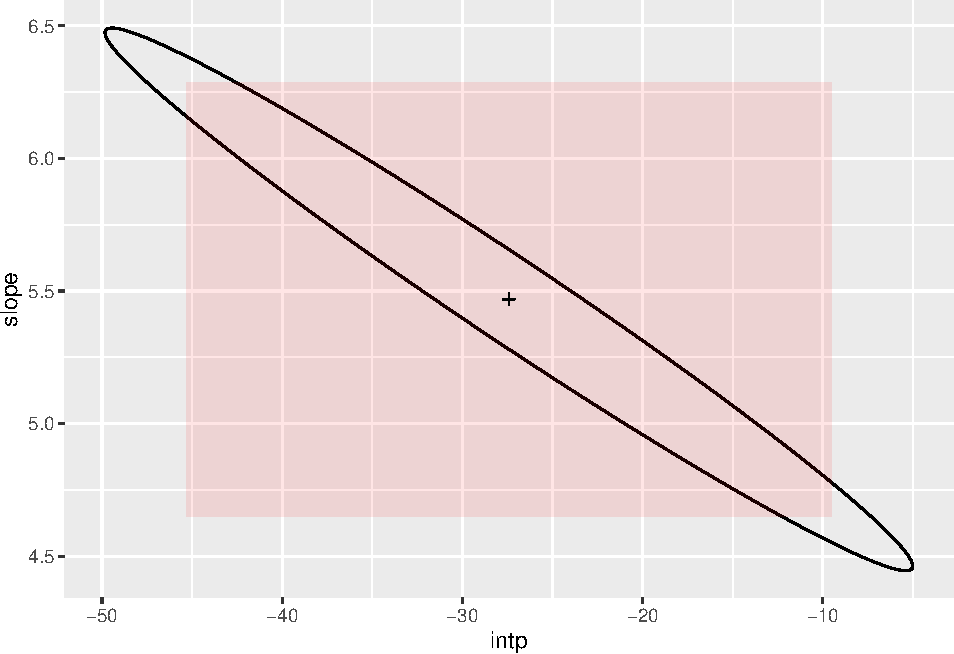
\includegraphics{TP-ML-Regression_files/figure-latex/unnamed-chunk-17-1.pdf}

\hypertarget{ruxe9gression-linuxe9aire-multiple}{%
\section{Régression linéaire
multiple}\label{ruxe9gression-linuxe9aire-multiple}}

Dans cette partie, nous souhaitons analyser la relation entre le maximum
journalier de la concentration d'ozone (maxO3) et

\begin{itemize}
\tightlist
\item
  la température à différentes heures de la journée (T9, T12, T15),
\item
  la nébulosité à différentes heures de la journée (Ne9, Ne12, Ne15),
\item
  la projection du vent sur l'axe Est-Ouest à différentes heures de la
  journée (Vx9, Vx12,Vx15),
\item
  la concentration maximale d'ozone de la veille (maxO3v)
\end{itemize}

On va donc utiliser le sous-jeu de données suivant

\begin{Shaded}
\begin{Highlighting}[]
\NormalTok{ozone1 }\OtherTok{=}\NormalTok{ ozone[,}\DecValTok{1}\SpecialCharTok{:}\DecValTok{11}\NormalTok{]}
\end{Highlighting}
\end{Shaded}

et mettre en place un modèle de régression linéaire multiple.

\begin{enumerate}
\def\labelenumi{\arabic{enumi}.}
\tightlist
\item
  Faites une analyse descriptive de ce jeu de données.
\end{enumerate}

\begin{Shaded}
\begin{Highlighting}[]
\CommentTok{\# A COMPLETER}
\end{Highlighting}
\end{Shaded}

\begin{enumerate}
\def\labelenumi{\arabic{enumi}.}
\setcounter{enumi}{1}
\tightlist
\item
  Rappelez l'écriture mathématique du modèle de régression linéaire
  multiple.
\end{enumerate}

Matriciellement, le modèle s'écrit : \[
Y = X\theta + \varepsilon 
\] avec \(X \in \mathcal{M}_{n,k}(\mathbb{R})\),
\(\theta \in \mathcal{M}_{k,1}(\mathbb{R})\) (partie déterministe) et
\(\varepsilon\)

\begin{enumerate}
\def\labelenumi{\arabic{enumi}.}
\setcounter{enumi}{2}
\tightlist
\item
  Ajustez un modèle de régression linéaire multiple à l'aide de la
  commande \texttt{lm()} et commentez les résultats (on appelle reg.mul
  la sortie de R dans la suite).
\end{enumerate}

\begin{Shaded}
\begin{Highlighting}[]
\NormalTok{reg.mul }\OtherTok{=} \FunctionTok{lm}\NormalTok{( ... ) }\CommentTok{\# A COMPLETER}
\NormalTok{resume.mul }\OtherTok{=} \FunctionTok{summary}\NormalTok{(reg.mul)}
\FunctionTok{summary}\NormalTok{(reg.mul)}
\end{Highlighting}
\end{Shaded}

\begin{enumerate}
\def\labelenumi{\arabic{enumi}.}
\setcounter{enumi}{3}
\tightlist
\item
  Etudiez les résidus
\end{enumerate}

\begin{Shaded}
\begin{Highlighting}[]
\CommentTok{\# COMPLETER}
\end{Highlighting}
\end{Shaded}

\hypertarget{suxe9lection-de-variables}{%
\section{Sélection de variables}\label{suxe9lection-de-variables}}

Dans le \texttt{summary(reg.mul)}, un test est fait sur chaque
coefficient. Il revient à tester que la variable n'apporte pas
d'information supplémentaire sachant que toutes les autres variables
sont dans le modèle. Il est donc préférable d'utiliser des procédures de
choix de modèles pour sélectionner les variables significatives. On va
ici comparer la sélection de variable obtenue par différents critères:
BIC, AIC, \(R^2\) ajusté, Cp de Mallows. Pour cela, vous pouvez utiliser
la fonction \texttt{regsubsets()} de la librairie \emph{leaps} et la
fonction \texttt{stepAIC()} de la librairie \emph{MASS}. Commentez les
résultats obtenus avec les différents critères, vous pourrez vous aider
des commandes suivantes :

\begin{Shaded}
\begin{Highlighting}[]
\NormalTok{choix}\OtherTok{=}\FunctionTok{regsubsets}\NormalTok{(...) }\CommentTok{\# A COMPLETER}
\FunctionTok{stepAIC}\NormalTok{(...)}
\CommentTok{\# A COMPLETER}
\end{Highlighting}
\end{Shaded}

Avec le critère BIC, nous retenons 4 variables : T12, Ne9, Vx9 et
maxO3v.\\
A l'aide des commandes suivantes, testez le sous-modèle avec les 4
variables retenues par BIC contre le modèle complet. Commentez.

\begin{Shaded}
\begin{Highlighting}[]
\NormalTok{reg.fin}\OtherTok{=}\FunctionTok{lm}\NormalTok{(maxO3}\SpecialCharTok{\textasciitilde{}}\NormalTok{T12}\SpecialCharTok{+}\NormalTok{Ne9}\SpecialCharTok{+}\NormalTok{Vx9}\SpecialCharTok{+}\NormalTok{maxO3v,}\AttributeTok{data=}\NormalTok{ozone1)}
\FunctionTok{summary}\NormalTok{(reg.fin)}
\FunctionTok{anova}\NormalTok{(reg.fin,reg.mul)}
\end{Highlighting}
\end{Shaded}

\hypertarget{ruxe9gressions-ruxe9gularisuxe9es}{%
\section{Régressions
régularisées}\label{ruxe9gressions-ruxe9gularisuxe9es}}

On commence par centrer et réduire les données avant de mettre en place
et comparer des méthodes de régression régularisées.

\begin{Shaded}
\begin{Highlighting}[]
\NormalTok{tildeY}\OtherTok{=}\FunctionTok{scale}\NormalTok{(ozone1[,}\DecValTok{1}\NormalTok{],}\AttributeTok{center=}\NormalTok{T,}\AttributeTok{scale=}\NormalTok{T)}
\NormalTok{tildeX}\OtherTok{=}\FunctionTok{scale}\NormalTok{(ozone1[,}\SpecialCharTok{{-}}\DecValTok{1}\NormalTok{],}\AttributeTok{center=}\NormalTok{T,}\AttributeTok{scale=}\NormalTok{T)}
\end{Highlighting}
\end{Shaded}

\hypertarget{ruxe9gression-ridge}{%
\subsection{Régression Ridge}\label{ruxe9gression-ridge}}

\begin{enumerate}
\def\labelenumi{\arabic{enumi}.}
\tightlist
\item
  A l'aide de la fonction \texttt{glmnet()}, ajustez une régression
  ridge en faisant varier \(\lambda\) sur une grille. On stockera le
  résultat dans la variable \texttt{fitridge}. Explorez le contenu de
  \texttt{fitridge}.
\end{enumerate}

\begin{Shaded}
\begin{Highlighting}[]
\NormalTok{lambda\_seq}\OtherTok{\textless{}{-}}\DecValTok{10}\SpecialCharTok{\^{}}\NormalTok{(}\FunctionTok{seq}\NormalTok{(}\SpecialCharTok{{-}}\DecValTok{4}\NormalTok{,}\DecValTok{4}\NormalTok{,}\FloatTok{0.01}\NormalTok{))}
\NormalTok{fitridge }\OtherTok{\textless{}{-}} \FunctionTok{glmnet}\NormalTok{(...) }\CommentTok{\# A completer}
\FunctionTok{summary}\NormalTok{(fitridge)}
\end{Highlighting}
\end{Shaded}

\begin{enumerate}
\def\labelenumi{\arabic{enumi}.}
\setcounter{enumi}{1}
\tightlist
\item
  Tracez les chemins de régularisation de chaque variable et commentez.
\end{enumerate}

\begin{Shaded}
\begin{Highlighting}[]
\NormalTok{df}\OtherTok{=}\FunctionTok{data.frame}\NormalTok{(}\AttributeTok{lambda =} \FunctionTok{rep}\NormalTok{(fitridge}\SpecialCharTok{$}\NormalTok{lambda,}\FunctionTok{ncol}\NormalTok{(tildeX)), }\AttributeTok{theta=}\FunctionTok{as.vector}\NormalTok{(}\FunctionTok{t}\NormalTok{(fitridge}\SpecialCharTok{$}\NormalTok{beta)),}\AttributeTok{variable=}\FunctionTok{rep}\NormalTok{(}\FunctionTok{colnames}\NormalTok{(tildeX),}\AttributeTok{each=}\FunctionTok{length}\NormalTok{(fitridge}\SpecialCharTok{$}\NormalTok{lambda)))}
\NormalTok{g1 }\OtherTok{=} \FunctionTok{ggplot}\NormalTok{(df,}\FunctionTok{aes}\NormalTok{(}\AttributeTok{x=}\NormalTok{lambda,}\AttributeTok{y=}\NormalTok{theta,}\AttributeTok{col=}\NormalTok{variable))}\SpecialCharTok{+}
  \FunctionTok{geom\_line}\NormalTok{()}\SpecialCharTok{+}
  \FunctionTok{theme}\NormalTok{(}\AttributeTok{legend.position=}\StringTok{"bottom"}\NormalTok{)}\SpecialCharTok{+}
  \FunctionTok{scale\_x\_log10}\NormalTok{()}
\FunctionTok{ggplotly}\NormalTok{(g1)}
\end{Highlighting}
\end{Shaded}

\begin{enumerate}
\def\labelenumi{\arabic{enumi}.}
\setcounter{enumi}{2}
\tightlist
\item
  A l'aide de la fonction \texttt{cv.glmnet()} mettez en place une
  validation croisée pour sélectionner le ``meilleur'' \(\lambda\) par
  MSE.
\end{enumerate}

\begin{Shaded}
\begin{Highlighting}[]
\NormalTok{ridge\_cv }\OtherTok{\textless{}{-}} \FunctionTok{cv.glmnet}\NormalTok{(...) }\CommentTok{\# A completer}
\NormalTok{best\_lambda }\OtherTok{\textless{}{-}}\NormalTok{ ridge\_cv}\SpecialCharTok{$}\NormalTok{lambda.min}
\end{Highlighting}
\end{Shaded}

\begin{Shaded}
\begin{Highlighting}[]
\NormalTok{df2}\OtherTok{=}\FunctionTok{data.frame}\NormalTok{(}\AttributeTok{lambda=}\NormalTok{ridge\_cv}\SpecialCharTok{$}\NormalTok{lambda,}\AttributeTok{MSE=}\NormalTok{ridge\_cv}\SpecialCharTok{$}\NormalTok{cvm,}\AttributeTok{cvup=}\NormalTok{ridge\_cv}\SpecialCharTok{$}\NormalTok{cvup,}\AttributeTok{cvlo=}\NormalTok{ridge\_cv}\SpecialCharTok{$}\NormalTok{cvlo)}
\NormalTok{gmse}\OtherTok{\textless{}{-}}\FunctionTok{ggplot}\NormalTok{(df2)}\SpecialCharTok{+}
  \FunctionTok{geom\_line}\NormalTok{(}\FunctionTok{aes}\NormalTok{(}\AttributeTok{x=}\NormalTok{lambda,}\AttributeTok{y=}\NormalTok{MSE))}\SpecialCharTok{+}
  \FunctionTok{geom\_vline}\NormalTok{(}\AttributeTok{xintercept =}\NormalTok{ ridge\_cv}\SpecialCharTok{$}\NormalTok{lambda.min,}\AttributeTok{col=}\StringTok{"red"}\NormalTok{,}\AttributeTok{linetype=}\StringTok{"dotted"}\NormalTok{)}\SpecialCharTok{+}
  \FunctionTok{geom\_line}\NormalTok{(}\FunctionTok{aes}\NormalTok{(}\AttributeTok{x=}\NormalTok{lambda,}\AttributeTok{y=}\NormalTok{cvup),}\AttributeTok{col=}\StringTok{"blue"}\NormalTok{,}\AttributeTok{linetype=}\StringTok{"dotted"}\NormalTok{)}\SpecialCharTok{+}
  \FunctionTok{geom\_line}\NormalTok{(}\FunctionTok{aes}\NormalTok{(}\AttributeTok{x=}\NormalTok{lambda,}\AttributeTok{y=}\NormalTok{cvlo),}\AttributeTok{col=}\StringTok{"blue"}\NormalTok{,}\AttributeTok{linetype=}\StringTok{"dotted"}\NormalTok{)}\SpecialCharTok{+}
  \CommentTok{\#xlim(c(0,ridge\_cv$lambda.min+0.5))+}
  \FunctionTok{scale\_x\_log10}\NormalTok{()}
\FunctionTok{ggplotly}\NormalTok{(gmse)}
\end{Highlighting}
\end{Shaded}

La valeur de \(\lambda\) sélectionnée vaut \ldots.

\begin{Shaded}
\begin{Highlighting}[]
\NormalTok{g1}\OtherTok{=}\NormalTok{g1 }\SpecialCharTok{+} 
  \FunctionTok{geom\_vline}\NormalTok{(}\AttributeTok{xintercept =}\NormalTok{ best\_lambda,}\AttributeTok{linetype=}\StringTok{"dotted"}\NormalTok{, }\AttributeTok{color =} \StringTok{"red"}\NormalTok{)}\SpecialCharTok{+}
  \FunctionTok{scale\_x\_log10}\NormalTok{()}
\end{Highlighting}
\end{Shaded}

\hypertarget{ruxe9gression-lasso}{%
\subsection{Régression Lasso}\label{ruxe9gression-lasso}}

\begin{enumerate}
\def\labelenumi{\arabic{enumi}.}
\tightlist
\item
  A l'aide de la fonction \texttt{glmnet()}, ajustez une régression
  Lasso en faisant varier \(\lambda\) sur une grille. On stockera le
  résultat dans la variable \texttt{fitlasso}. Explorez le contenu de
  \texttt{fitlasso}.
\end{enumerate}

\begin{Shaded}
\begin{Highlighting}[]
\NormalTok{fitlasso }\OtherTok{\textless{}{-}} \FunctionTok{glmnet}\NormalTok{(...) }\CommentTok{\# A COMPLETER}
\FunctionTok{summary}\NormalTok{(fitlasso)}
\end{Highlighting}
\end{Shaded}

\begin{enumerate}
\def\labelenumi{\arabic{enumi}.}
\setcounter{enumi}{1}
\tightlist
\item
  Tracez le chemin de régularisation de chacune des variables et
  commentez
\end{enumerate}

\begin{Shaded}
\begin{Highlighting}[]
\NormalTok{df}\OtherTok{=}\FunctionTok{data.frame}\NormalTok{(}\AttributeTok{lambda =} \FunctionTok{rep}\NormalTok{(fitlasso}\SpecialCharTok{$}\NormalTok{lambda,}\FunctionTok{ncol}\NormalTok{(tildeX)), }\AttributeTok{theta=}\FunctionTok{as.vector}\NormalTok{(}\FunctionTok{t}\NormalTok{(fitlasso}\SpecialCharTok{$}\NormalTok{beta)),}\AttributeTok{variable=}\FunctionTok{rep}\NormalTok{(}\FunctionTok{colnames}\NormalTok{(tildeX),}\AttributeTok{each=}\FunctionTok{length}\NormalTok{(fitlasso}\SpecialCharTok{$}\NormalTok{lambda)))}
\NormalTok{g3 }\OtherTok{=} \FunctionTok{ggplot}\NormalTok{(df,}\FunctionTok{aes}\NormalTok{(}\AttributeTok{x=}\NormalTok{lambda,}\AttributeTok{y=}\NormalTok{theta,}\AttributeTok{col=}\NormalTok{variable))}\SpecialCharTok{+}
  \FunctionTok{geom\_line}\NormalTok{()}\SpecialCharTok{+}
  \FunctionTok{theme}\NormalTok{(}\AttributeTok{legend.position=}\StringTok{"bottom"}\NormalTok{)}\SpecialCharTok{+}
  \FunctionTok{scale\_x\_log10}\NormalTok{()}
\FunctionTok{ggplotly}\NormalTok{(g3)}
\end{Highlighting}
\end{Shaded}

\begin{enumerate}
\def\labelenumi{\arabic{enumi}.}
\setcounter{enumi}{2}
\tightlist
\item
  A l'aide de la fonction \texttt{cv.glmnet()} mettez en place une
  validation croisée pour sélectionner le ``meilleur'' \(\lambda\) par
  MSE. En pratique, il est préconisé d'utilisé \texttt{lambda.1se} (la
  plus grande valeur de \(\lambda\) telle que l'erreur standard se situe
  à moins de 1 de celle du minimum).
\end{enumerate}

\begin{Shaded}
\begin{Highlighting}[]
\NormalTok{lasso\_cv }\OtherTok{\textless{}{-}} \FunctionTok{cv.glmnet}\NormalTok{(...) }\CommentTok{\# A COMPLETER}
\NormalTok{best\_lambda }\OtherTok{\textless{}{-}}\NormalTok{lasso\_cv}\SpecialCharTok{$}\NormalTok{lambda.min}
\NormalTok{lambda1se }\OtherTok{\textless{}{-}}\NormalTok{ lasso\_cv}\SpecialCharTok{$}\NormalTok{lambda}\FloatTok{.1}\NormalTok{se}
\end{Highlighting}
\end{Shaded}

La valeur de \(\lambda\) sélectionnée vaut \ldots.

\begin{Shaded}
\begin{Highlighting}[]
\NormalTok{g3}\OtherTok{=}\NormalTok{g3 }\SpecialCharTok{+} 
  \FunctionTok{geom\_vline}\NormalTok{(}\AttributeTok{xintercept =}\NormalTok{ best\_lambda,}\AttributeTok{linetype=}\StringTok{"dotted"}\NormalTok{, }\AttributeTok{color =} \StringTok{"red"}\NormalTok{)}\SpecialCharTok{+}
  \FunctionTok{geom\_vline}\NormalTok{(}\AttributeTok{xintercept =}\NormalTok{ lambda1se,}\AttributeTok{linetype=}\StringTok{"dotted"}\NormalTok{, }\AttributeTok{color =} \StringTok{"blue"}\NormalTok{)}\SpecialCharTok{+}
  \FunctionTok{scale\_x\_log10}\NormalTok{()}
\NormalTok{g3}
\end{Highlighting}
\end{Shaded}

\begin{enumerate}
\def\labelenumi{\arabic{enumi}.}
\setcounter{enumi}{3}
\tightlist
\item
  Quelle sélection de variables obtient-on alors ?
\end{enumerate}

Vous pouvez utiliser la fonction \texttt{extract.coef()} de la librairie
\texttt{coefplot}

\begin{Shaded}
\begin{Highlighting}[]
\CommentTok{\# A COMPLETER}
\end{Highlighting}
\end{Shaded}

\hypertarget{ruxe9gression-elastic-net}{%
\subsection{Régression Elastic Net}\label{ruxe9gression-elastic-net}}

\begin{enumerate}
\def\labelenumi{\arabic{enumi}.}
\tightlist
\item
  Reprenez les questions précédentes pour ajuster une régression Elastic
  Net
\end{enumerate}

\begin{Shaded}
\begin{Highlighting}[]
\NormalTok{fitEN }\OtherTok{\textless{}{-}} \FunctionTok{glmnet}\NormalTok{(...)}
\NormalTok{df}\OtherTok{=}\FunctionTok{data.frame}\NormalTok{(}\AttributeTok{lambda =} \FunctionTok{rep}\NormalTok{(fitEN}\SpecialCharTok{$}\NormalTok{lambda,}\FunctionTok{ncol}\NormalTok{(tildeX)), }\AttributeTok{theta=}\FunctionTok{as.vector}\NormalTok{(}\FunctionTok{t}\NormalTok{(fitEN}\SpecialCharTok{$}\NormalTok{beta)),}\AttributeTok{variable=}\FunctionTok{rep}\NormalTok{(}\FunctionTok{c}\NormalTok{(}\FunctionTok{colnames}\NormalTok{(tildeX)),}\AttributeTok{each=}\FunctionTok{length}\NormalTok{(fitEN}\SpecialCharTok{$}\NormalTok{lambda)))}
\NormalTok{g4 }\OtherTok{=} \FunctionTok{ggplot}\NormalTok{(df,}\FunctionTok{aes}\NormalTok{(}\AttributeTok{x=}\NormalTok{lambda,}\AttributeTok{y=}\NormalTok{theta,}\AttributeTok{col=}\NormalTok{variable))}\SpecialCharTok{+}
  \FunctionTok{geom\_line}\NormalTok{()}\SpecialCharTok{+}
  \FunctionTok{theme}\NormalTok{(}\AttributeTok{legend.position=}\StringTok{"bottom"}\NormalTok{)}\SpecialCharTok{+}
  \FunctionTok{scale\_x\_log10}\NormalTok{()}
\end{Highlighting}
\end{Shaded}

\begin{Shaded}
\begin{Highlighting}[]
\NormalTok{EN\_cv }\OtherTok{\textless{}{-}} \FunctionTok{cv.glmnet}\NormalTok{(...) }\CommentTok{\# A COMPLETER}
\NormalTok{best\_lambda }\OtherTok{\textless{}{-}}\NormalTok{EN\_cv}\SpecialCharTok{$}\NormalTok{lambda.min}
\NormalTok{g4}\OtherTok{=}\NormalTok{g4 }\SpecialCharTok{+} \FunctionTok{geom\_vline}\NormalTok{(}\AttributeTok{xintercept =}\NormalTok{ best\_lambda,}\AttributeTok{linetype=}\StringTok{"dotted"}\NormalTok{, }
                \AttributeTok{color =} \StringTok{"red"}\NormalTok{)}
\FunctionTok{ggplotly}\NormalTok{(g4)}
\end{Highlighting}
\end{Shaded}

\begin{enumerate}
\def\labelenumi{\arabic{enumi}.}
\setcounter{enumi}{1}
\tightlist
\item
  Comparez les coefficients obtenus avec la régression linéaire, la
  régression ridge, la régression Lasso et la régression ElasticNet
\end{enumerate}

\end{document}
